\chapter{Implementación}
\label{cap:implementacion}

Tras haber dedicado los capítulos anteriores a analizar detalladamente los fundamentos teóricos 
y las distintas variantes de la arquitectura del transformador, el siguiente paso lógico es su aplicación práctica. 
Además surge la curiosidad de ver cómo se comporta el modelo cuando se enfrenta a una tarea real y compleja. 
Por este motivo, el núcleo de este capítulo se centra en la implementación de un transformador de tipo 
codificador-decodificador, diseñado específicamente para traducir frases del inglés al español.

Este capítulo tiene como objetivo describir todo el proceso de desarrollo de forma estructurada. 
Para ello, se abordarán los detalles técnicos que han hecho posible el entrenamiento del modelo, empezando por la 
selección y limpieza del conjunto de datos empleado. 
También se detallarán los hiperparámetros que definen la estructura de la red y otros criterios de diseño que, aunque 
no se incluyeron en la parte teórica para no desviar la atención, resultan fundamentales para que el sistema funcione 
correctamente en la práctica.

En la actualidad, existen numerosas librerías que permiten importar modelos pre-entrenados o utilizar 
arquitecturas ya implementadas con apenas unas pocas líneas de código. Sin embargo, dado que el propósito de este 
trabajo es pedagógico y analítico, se ha optado por prescindir de estas herramientas de alto nivel y programar el 
traductor íntegramente desde cero utilizando Python y la librería científica PyTorch. Esta decisión permite profundizar 
en los mecanismos internos del sistema y comprender de primera mano todos los detalles técnicos  que son fundamentales 
para el correcto funcionamiento del modelo.

Finalmente, para facilitar la reproducción del experimento y la transparencia del trabajo, el código fuente y 
la estructura del proyecto están disponibles en un repositorio 
público de \href{https://github.com/skaczylo/Transformer-Translator}{\textcolor{blue}{GitHub}}. 
Allí se incluye también todo lo necesario para configurar el entorno fácilmente en una sola línea de comando y 
probar el funcionamiento del modelo mediante una interfaz donde el usuario puede introducir frases en inglés 
de forma sencilla y observar la traducción generada por el sistema.


\section{Conjunto de datos: OPUS100}

Para el desarrollo de cualquier modelo de aprendizaje automático, el primer paso fundamental consiste en la obtención y 
preparación de un conjunto de datos inicial. En nuestro caso, al tratarse de un sistema de traducción de inglés a español, 
es imprescindible disponer de un corpus compuesto por pares de frases traducidas con precisión. 
Para este propósito, se ha seleccionado el conjunto de datos OPUS100 \cite{TIEDEMANN12.463}: un corpus de 
traducción de inglés a $100$ idiomas distintos\footnote{Al principio, durante el desarrollo del proyecto, se empleó otro conjunto de datos. 
No obstante, tras varias pruebas se observó que los datos eran de muy mala calidad pues las traducciones apenas tenían sentido y 
muchas de ellas tenían datos ``basura''.}. En nuestro caso, solo utilizaremos aquellas frases traducidas de inglés a 
español\footnote{Todo el código correspondiente al procesamiento y tratamiento del conjunto de datos se encuentra detallado en el 
archivo \texttt{notebooks/dataset.ipynb}.}.

Este corpus se estructura en tres subconjuntos diferenciados que permiten gestionar las distintas fases del desarrollo:

\begin{itemize}
    \item \textbf{Conjunto de entrenamiento}: 1.000.000 de pares de frases, destinados al ajuste de los parámetros y pesos de la red.
    \item \textbf{Conjunto de validación}: 2.000 pares de frases, utilizados para supervisar el rendimiento durante el entrenamiento y 
    evitar el sobreajuste.
    \item \textbf{Conjunto de prueba}: 2.000 pares de frases, reservados para la evaluación final del modelo en un entorno no visto.
\end{itemize}

Destacar que, aunque a priori el tamaño del conjunto seleccionado pueda parecer considerable, su escala resulta modesta al compararse con 
los grandes sistemas de traducción desarrollados por entidades como Google. 
Estos modelos han sido entrenados con un volumen aproximado 
de 25.000 millones de pares de datos, tal y como se analiza en el artículo 
\textit{Massively Multilingual Neural Machine Translation in the Wild: Findings and Challenges} \cite{aharoni-etal-2019-massively}. 
Otro ejemplo sería el modelo de traducción del artículo \textit{Atention is all you need} \cite{vaswani2017attention_arxiv}
donde se utilizó un conjunto de datos de 36 millones de pares de frases traducidas. 

\subsection{Filtrado y calidad de los datos}

En el ámbito de la inteligencia artificial, la eficacia de la arquitectura depende también de la calidad de la información con la que se entrena. 
Por ello, se ha diseñado un proceso de filtrado  para eliminar el ruido y las inconsistencias  en el conjunto original:

\begin{enumerate}
    \item \textbf{Limpieza de datos nulos}: Se han descartado todas las entradas que contengan valores nulos o donde alguna de las cadenas de 
    texto (inglesa o española) esté vacía.
    \item \textbf{Longitud mínima}: Se han eliminado aquellas traducciones en las que alguna de las frases posea menos de tres palabras, 
    con el fin de asegurar un mínimo de carga semántica.
    \item \textbf{Detección de anomalías}: Se han filtrado aquellos casos extraños donde la traducción al español resulta ser una 
    copia exacta de la frase original en inglés.
\end{enumerate}


Además, para garantizar la coherencia lingüística de los pares, hemos definido una métrica denominada \textit{ratio} ($r$). 
Este valor se define como el cociente entre la longitud de la frase de salida y la de entrada:
\begin{equation}
    r = \frac{L_{es}}{L_{en}}
\end{equation}
donde $L_{es}$ es la longitud de la frase en español y $L_{en}$ es la longitud de la frase en inglés\footnote{Aquí, longitud de la frase 
hace referencia al número de palabras que componen la frase.}.
Es razonable esperar que las extensiones de las frases no difieran de manera excesiva. Un ratio superior a 2 indicaría que la 
traducción emplea más del doble de palabras que el original, lo cual resulta anómalo en nuestro dominio. Por otro lado, un valor inferior 
a 0,5 sugeriría una pérdida significativa de información o una traducción incompleta. 
Por tanto, se ha optado por conservar únicamente aquellas traducciones cuyo ratio se encuentre dentro del intervalo $(\frac{1}{2}, 2)$.

Finalmente, y tras aplicar el filtrado, el conjunto de entrenamiento se reduce a 759.856 traducciones, es decir, se han
 descartado un total de  240.144 traducciones del conjunto inicial.

\subsection{Estructura de los datos}

Tras descartar los datos de baja calidad, conviene estudiar la estructura y las características de los datos que componen el corpus. 
Este análisis permite comprender la distribución de las longitudes y el ratio de las secuencias. Para ello, 
se han calculado la media, la desviación típica y los percentiles del 25\%, 50\%, 75\%, 90\% y 95\% sobre la longitud de las frases y su ratio, 
obteniendo los resultados que se muestran en la Tabla \ref{tab:estadisticas_corpus}. Asimismo, 
para obtener una perspectiva más intuitiva de cómo se organizan o reparten los datos, se puede observar 
la distribución de estas mediante los histogramas presentados en la figura \ref{fig:histogramas}.

\begin{table}[t]
\centering
\begin{tabular}{lccc}
\hline
\textbf{Estadístico} & \textbf{$L_{en}$} & \textbf{$L_{es}$} & \textbf{$r$} \\ \hline
Media                & 12,94             & 13,46             & 1,02                 \\
Desviación típica    & 13,21             & 14,84             & 0,24                 \\
Mínimo               & 3,00              & 3,00              & 0,50                 \\
25\%                 & 5,00              & 5,00              & 0,83                 \\
50\%                 & 8,00              & 8,00              & 1,00                 \\
75\%                 & 16,00             & 16,00             & 1,17                 \\
90\%                 & 28,00             & 31,00             & 1,33                 \\
95\%                 & 38,00             & 43,00             & 1,45                 \\
Máximo               & 1737,00           & 1721,00           & 1,98                 \\ \hline
\end{tabular}
\caption{Estadísticas descriptivas del corpus filtrado para las longitudes en inglés ($L_{en}$), español ($L_{es}$) y el ratio ($r$).}
\label{tab:estadisticas_corpus}
\end{table}

\begin{figure}[t!] 
    \centering       
    % --- HISTOGRAMA INGLÉS ---
    \subfloat[Distribución de la longitud en inglés ($L_{en}$).\label{subfig:hist_en}]{
        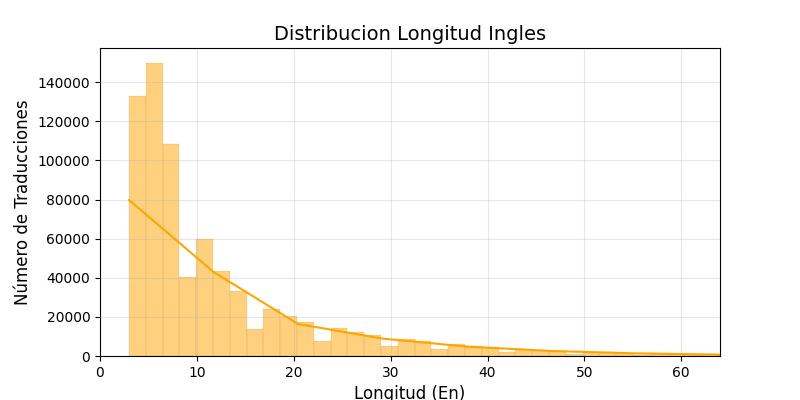
\includegraphics[width=0.7\textwidth]{Imagenes/histograma_lon_en.png}
    } 
    \hfill
    % --- HISTOGRAMA ESPAÑOL ---
    \subfloat[Distribución de la longitud en español ($L_{es}$).\label{subfig:hist_es}]{
        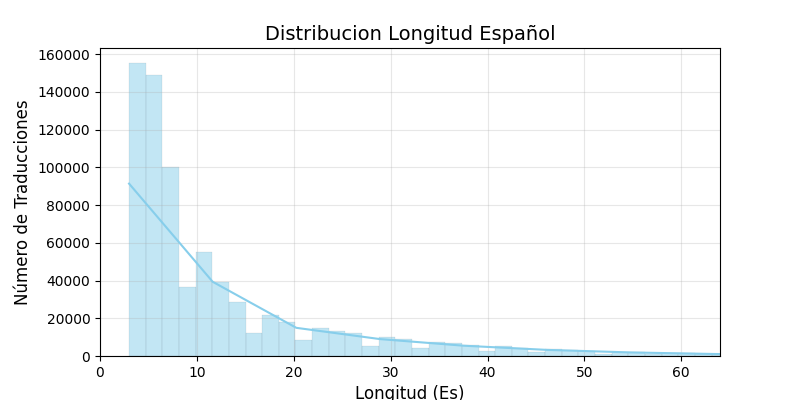
\includegraphics[width=0.7\textwidth]{Imagenes/histograma_lon_es.png}
    }

    \vspace{1em} % Espacio vertical entre filas

    % --- HISTOGRAMA RATIO ---
    \subfloat[Distribución del ratio ($r$).\label{subfig:hist_ratio}]{
        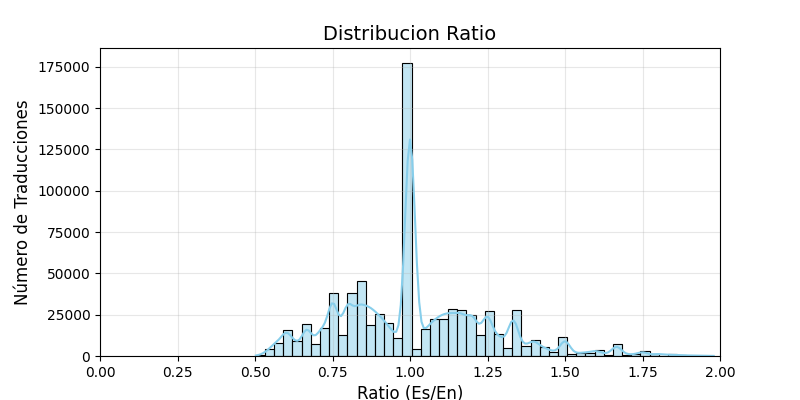
\includegraphics[width=0.7\textwidth]{Imagenes/histograma_ratio.png}
    }

    \caption{Histogramas de frecuencias para las longitudes de las frases en ambos idiomas y la distribución del ratio de traducción en el 
    corpus filtrado.}
    \label{fig:histogramas} 
\end{figure}

Se observa que, aunque el rango de longitudes es amplio, el 90\% de las frases en español poseen 31 palabras o menos. 
El ratio medio de 1,02  garantiza un conjunto de datos equilibrado para el proceso de aprendizaje.

Otro punto de interés reside en los valores máximos registrados, que ascienden a 1.737 palabras en inglés y 1.721 en español. 
Se observa una diferencia sustancial con la tendencia mayoritaria, ya que el 95\% de las frases contiene 43 palabras o menos. 
Por este motivo, y en previsión del número $N$ de \textit{tokens} que el transformador será capaz de procesar y que se detallará más 
adelante, se ha optado por descartar aquellas frases cuya longitud exceda las 64 palabras. Se han eliminado 10.753 pares de frases y, finalmente, 
el corpus resultante está formado por 749.103 traducciones.

Para completar el estudio descriptivo, resulta útil e interesante evaluar la amplitud del vocabulario en ambos idiomas, es decir, 
cuantificar la cantidad de palabras distintas que el modelo encontrará durante el entrenamiento. En la Tabla \ref{tab:palabras_unicas} 
se detallan los resultados obtenidos para cada lengua donde se observa que el español presenta un número significativamente mayor de 
palabras únicas en comparación con el inglés. Sin embargo, esto no es un problema y, en cierto sentido, es razonable esa diferencia. 
Uno de los motivos es, por ejemplo, la forma de conjugar verbos: en inglés el verbo no suele cambiar mucho a diferencia del español que 
tiene decenas de formas distintas según el tiempo, la persona y el número. Otro motivo es que los adjetivos en inglés 
son invariables: la palabra ``red'' sirve para describir cualquier objeto sin importar género o cantidad; en cambio, en español esa misma 
palabra se divide en cuatro formas distintas ``rojo'', ``roja'', ``rojos'' y ``rojas''.

\begin{table}[t]
\centering
\begin{tabular}{lc}
\hline
\textbf{Idioma} & \textbf{Total de palabras únicas} \\ \hline
Inglés          & 152.068                           \\
Español         & 208.369                           \\ \hline
\end{tabular}
\caption{Riqueza léxica del corpus expresada en número de vocablos distintos.}
\label{tab:palabras_unicas}
\end{table}


También se ha realizado un análisis de las frecuencias de aparición para identificar las palabras predominantes en el corpus. 
En la Tabla \ref{tab:frecuencias} se recogen las diez palabras más frecuentes para cada idioma. 

\begin{table}[t]
\centering
\begin{tabular}{ccccc}
\hline
\textbf{Rango} & \textbf{Palabra (EN)} & \textbf{Frecuencia (EN)} & \textbf{Palabra (ES)} & \textbf{Frecuencia (ES)} \\ \hline
1              & the                   & 532.625                  & de                    & 582.017                  \\
2              & of                    & 268.586                  & la                    & 331.605                  \\
3              & to                    & 249.572                  & que                   & 266.058                  \\
4              & and                   & 222.554                  & el                    & 237.683                  \\
5              & you                   & 182.139                  & en                    & 230.591                  \\
6              & i                     & 179.156                  & y                     & 218.430                  \\
7              & a                     & 174.868                  & a                     & 205.047                  \\
8              & in                    & 165.885                  & los                   & 142.553                  \\
9              & that                  & 114.410                  & no                    & 140.768                  \\
10             & it                    & 104.917                  & un                    & 101.677                  \\ \hline
\end{tabular}
\caption{Clasificación de las diez palabras más frecuentes identificadas en el corpus.}
\label{tab:frecuencias}
\end{table}

Los resultados confirman que las palabras más utilizadas en ambos idiomas pertenecen a la categoría de palabras 
funcionales (artículos, preposiciones y conjunciones). Estos términos, aunque carecen de un peso semántico específico por sí solos, 
son los encargados de articular la estructura sintáctica de las oraciones. Destaca la frecuencia de la palabra ``the'' en inglés y 
la preposición ``de'' en español, encabezando sus respectivos listados con una frecuencia considerablemente superior al resto de términos.


%==========================================
%VOCABULARIO
%==========================================
\section{Vocabulario}

Una vez tenemos los datos con los que entrenar el modelo, el siguiente paso crítico en la implementación es el diseño del vocabulario. 
Inicialmente se planteó el uso de un vocabulario ya creado como el empleado en la arquitectura GPT2; sin embargo, se concluyó que dicha 
aproximación resultaría contraproducente para los fines de este trabajo. Los modelos de propósito general se entrenan con corpus masivos 
que incluyen desde literatura hasta código de programación, lo que genera una distribución de \tokens{} muy alejada de nuestro conjunto de 
traducción. Es por ello que emplear un vocabulario ajeno podría provocar una fragmentación excesiva de las palabras comunes de nuestro dominio en 
múltiples \tokens{}. Esto no solo incrementaría la longitud de las secuencias de entrada, sino que perjudicaría al mecanismo de autoatención 
del modelo: sería, en cierto modo, como considerar un vocabulario compuesto únicamente por caracteres. 



Teniendo todo esto en cuenta, se ha optado por construir un vocabulario $\mathcal{V}$ propio mediante la aplicación del algoritmo BPE 
(algoritmo \ref{alg:bpe}) sobre el conjunto de entrenamiento, es decir, sobre la unión de las frases en inglés y sus correspondientes 
traducciones al español. Inicialmente, $\mathcal{V}$ se compone de los caracteres individuales de ambos alfabetos. 
No obstante, para garantizar la calidad del vocabulario resultante, se debieron definir ciertas precondiciones en el proceso de construcción.

El primer problema al aplicar el algoritmo BPE directamente sobre el texto fue la generación de \tokens{} demasiado largos, que llegaban a 
ser frases casi completas. Esto ocurría porque, al repetir el proceso, las secuencias más comunes acababan siendo palabras enteras ya unidas 
entre sí, lo que restaba flexibilidad al modelo a la hora de traducir ciertas frases. Para evitarlo, en lugar de procesar
todo el texto de seguido, decidimos aplicar el algoritmo palabra por palabra. De esta forma, si llamamos $\mathcal{T}$ al conjunto de todas las 
frases del corpus, el conjunto $\mathcal{S}$ sobre el que aplicamos BPE pasa a ser la unión de las palabras individuales que forman dichas frases:
\begin{equation}
    \mathcal{S} = \bigcup_{t_i \in \mathcal{T}} \{w : w \in t_i\}
\end{equation}
donde $w$ denota una palabra perteneciente a una frase $t$.
Con esta restricción, nos aseguramos de que los caracteres solo se unan dentro de una misma palabra y  evitamos que se formen \tokens{} 
que sean frases enteras. 

Sin embargo, al separar el texto en palabras individuales, apareció otro problema: la falta de espacios. 
El algoritmo perdía la conexión entre palabras y el modelo generaba frases bien escritas pero totalmente pegadas, como ``Elgatoestásobrelamesa''.
Para solucionarlo, modificamos la segmentación inicial añadiendo el carácter especial ``$\cdot$'' al principio de cada palabra para representar 
el espacio en blanco. Al meter este símbolo en el vocabulario desde el principio, el BPE pudo integrarlo en los \tokens{} más comunes. 
Por ejemplo, la frase ``El gato'' se procesa como ``El'' y ``$\cdot$gato''. Si el algoritmo decide que ``ga'' y ``to'' aparecen mucho, 
el vocabulario final incluirá los \tokens{} ``$\cdot$ga'' y ``to''. De este modo, el modelo reconstruye la palabra sabiendo que el primer 
fragmento indica el inicio de una palabra nueva tras un espacio. Esta técnica permite que el resultado final sea legible y que el transformador pueda 
descomponer palabras complejas en piezas con significado propio.

Finalmente, tras aplicar estos ajustes, el resultado es un vocabulario $\mathcal{V}$ de 16.000 \tokens{} que mezcla raíces, prefijos, sufijos y/o 
palabras enteras de ambos idiomas. 
En la figura \ref{fig:muestra_vocabulario} se puede ver una pequeña muestra de los \tokens{} que forman parte de este vocabulario final que
utilizará el modelo tanto para comprender las frases originales en inglés como para realizar las correspondientes traducciones al español.


\begin{figure}[t]
    \centering
    \begin{small}
    \begin{tabular}{rlp{0.5cm}rl}
    \toprule
    \textbf{ID} & \textbf{Token} & & \textbf{ID} & \textbf{Token} \\
    \midrule
    283 & \texttt{$\cdot$the} & & 316 & \texttt{$\cdot$que} \\
    311 & \texttt{ing} & & 348 & \texttt{ción} \\
    330 & \texttt{$\cdot$and} & & 412 & \texttt{$\cdot$para} \\
    433 & \texttt{$\cdot$with} & & 490 & \texttt{ión} \\
    510 & \texttt{ould} & & 663 & \texttt{$\cdot$está} \\
    795 & \texttt{$\cdot$would} & & 1754 & \texttt{miento} \\
    1051 & \texttt{$\cdot$people} & & 2086 & \texttt{$\cdot$nuestra} \\
    1105 & \texttt{$\cdot$new} & & 3694 & \texttt{$\cdot$gobierno} \\
    \bottomrule
    \end{tabular}
    \end{small}
    \caption{Muestra representativa de tokens extraídos del vocabulario. 
    El punto de multiplicación ($\cdot$) representa un espacio en blanco inicial, indicando que el token marca el comienzo de una palabra.
    }
    \label{fig:muestra_vocabulario}
\end{figure}

\section{Transformador}
Con el vocabulario listo y los datos procesados, el siguiente paso es configurar la arquitectura neuronal. Para este traductor, hemos 
seguido el diseño de codificador-decodificador propuesto en el artículo original \textit{Attention Is All You Need}. Aunque la estructura 
general es la misma que explicamos en la sección \ref{subsec:codificador_decoficador}, hay un detalle fundamental en el diagrama 
original (ver figura \ref{fig:transformer_arch}) que todavía no hemos analizado: la codificación posicional(\textit{positional encoding}). 
Decidimos posponer su explicación para no sobrecargar los capítulos teóricos anteriores, pero es una pieza clave para que el sistema funcione 
en la práctica\footnote{Todo el código correspondiente al modelo se encuentra en la carpeta \texttt{src}. 
La arquitectura implementada y su configuración están en \texttt{src/transformer.py}.}.

\begin{figure}[t]
    \centering
    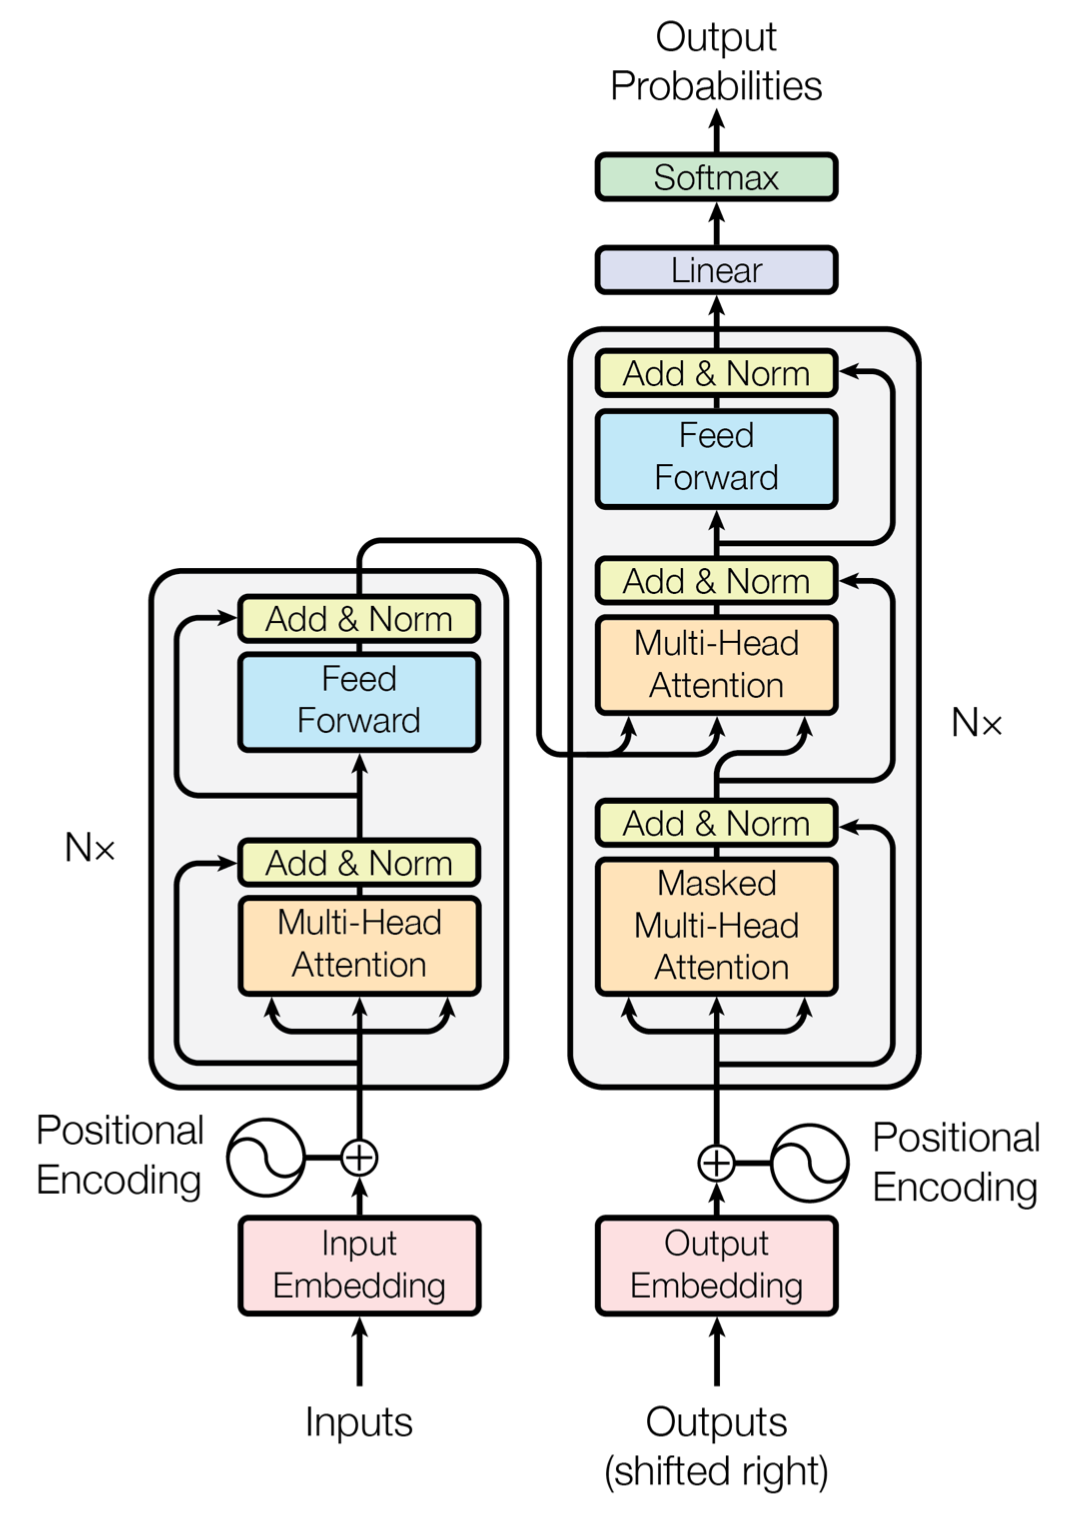
\includegraphics[width=0.55\textwidth]{Imagenes/attention_is_all_you_need.png}
    \caption{Imagen del artículo original donde se muestra la arquitectura del transformador.}
    \label{fig:transformer_arch}
\end{figure}


%==========================================
%POSITIONAL ENCODING
%==========================================
\subsection{Codificación posicional (\textit{Positional Encoding})}
Si analizamos cómo funciona el mecanismo de autoatención, veremos que carece por completo de una noción de orden secuencial pues al procesar 
todos los \tokens{} de forma paralela, el modelo es, por definición, invariante ante permutaciones. Sin embargo, en el lenguaje natural, el 
orden de las palabras es esencial para determinar el significado de la frase. Por ejemplo, no posee el mismo significado la frase 
\textit{``El perro mordió al hombre''} que \textit{``El hombre mordió al perro''}, a pesar de contener exactamente las mismas palabras.

Para integrar esta información de posición sin renunciar a las ventajas del procesamiento en paralelo, introducimos la codificación posicional 
(\textit{positional encoding}). 
El objetivo es asociar un vector de posición $\mathbf{r}_i$ a cada \token{} de entrada $\mathbf{x}_i$. Para ello sumaremos directamente 
el vector de posición al vector del \token{}:
\begin{equation}
    \widetilde{\mathbf{x}}_i = \mathbf{x}_i + \mathbf{r}_i
\end{equation}
obteniendo así un nuevo vector $\widetilde{\x}_i$ que codifica tanto la información del \token{} como su posición. Obviamente, para que esta 
operación sea posible es necesario que los vectores $\mathbf{r}_i$ tengan la misma dimensión $D_i$ que los \tokens{} $\x_n$. 
Existen diversas maneras de construir estos vectores $\{\mathbf{r}_i\}$. Una de las más conocidas es la basada en funciones sinusoidales de 
diferentes frecuencias, la cual permite que el modelo extrapole relaciones a secuencias de longitudes no 
vistas previamente (ver \cite[Cap 12]{Bishop:DeepLearning24} para más detalles). No obstante, para nuestra implementación hemos 
optado por el enfoque de codificaciones posicionales aprendidas donde definiremos una matriz de pesos posicionales, $\mathbf{\Omega_r}$ de 
dimensión $D_i \times N$, donde cada columna representa un vector de posición específico para cada una de las $N$ posiciones posibles:
\begin{equation}
    \mathbf{\Omega_r} = \begin{bmatrix} 
    | & | & & | \\ 
    \mathbf{r}_1 & \mathbf{r}_2 & \dots & \mathbf{r}_N \\ 
    | & | & & | 
    \end{bmatrix}
\end{equation}
Esta matriz irá ajustando sus valores durante el entrenamiento y, en consecuencia, el modelo aprenderá a determinar las posiciones 
de los \tokens{} que recibe como entrada.

%==========================================
%HIPERPARAMETROS
%==========================================
\subsection{Hiperparámetros}

Para ajustar el modelo a las características del corpus OPUS100 y a los recursos computacionales disponibles, se han definido los 
hiperparámetros que determinan la capacidad de aprendizaje y la complejidad estructural de la red:

\begin{itemize}
    \item \textbf{Dimensión de los \tokens{} ($D_i$):} 256. Representa la dimensionalidad de los \textit{tokens} que procesa el transformador o, 
    equivalentemente, la dimensión de los \textit{embeddings}.
    \item \textbf{Número de codificadores apilados:} 4.
    \item \textbf{Número de decodificadores apilados:} 4.
    \item \textbf{Capas de autoatención ($H$):} 8. Número de mecanismos de atención que trabajan simultáneamente en paralelo.
    \item \textbf{Número máximo de tokens ($N$):} 128. Define el número maximo de \tokens{} en los que se puede dividir una frase.
    \item \textbf{Cardinal del vocabulario ($k$):} 16.000. Tamaño total del diccionario de \textit{tokens} compartidos entre ambos idiomas.

\end{itemize}

Inicialmente se intentó aplicar la misma configuración que el artículo original 
\cite{vaswani2017attention_arxiv} donde se utilizaba la siguiente configuracion:
\begin{itemize}
    \item \textbf{Dimensión de los rasgos ($D_i$):} 512. 
    \item \textbf{Bloques transformadores apilados ($D$):} 6.
    \item \textbf{Capas de autoatención ($H$):} 8.
    \item \textbf{Número máximo de tokens ($N$):} 512.
    \item \textbf{Cardinal del vocabulario ($k$):} 37.000.
\end{itemize}

Sin embargo, y teniendo en cuenta que los recursos son limitados, se decidió reducirlos para que el proceso de entrenamiento no se alargase mucho. 
Además de que previamente se realizaron varias pruebas de entrenamiento donde se estimó el tiempo que tardaría en entrenar. 

\subsection{Entrenamiento}

Definidos los hiperparámetros pasamos a la fase de entrenamiento. Comentaremos detalles técnicos de esta fase siguiendo un poco la estructura 
del artículo original\footnote{Todo el código correspondiente al entrenamiento se encuentra detallado en el archivo \texttt{src/train.py} y 
la ejecución del mismo en  \texttt{notebooks/training\_colab.ipynb}.}.

\subsubsection{Hardware}
Se utilizó una tarjeta gráfica (GPU) NVIDIA A100 a través de la plataforma Google Colab y se entrenó durante 45 épocas\footnote{Una época es 
una pasada completa de todo el conjunto de datos de entrenamiento a través de la red neuronal.
En otras palabras, se completa una época cuando el modelo ha ``visto'' y procesado cada uno de los ejemplos de entrenamiento exactamente 
una vez para ajustar sus pesos y aprender de los errores cometidos.} dividiendo el conjunto total en lotes (\textit{batches}) de 128 traducciones. 
Cada época tardaba alrededor de unos 13 minutos y el entrenamiento total fueron en total $9$ horas aproximadamente.

\subsubsection{Criterio de Error y Función de Pérdida}

En este modelo se ha empleado la entropía cruzada (\textit{Cross Entropy}), ya que resulta la métrica óptima para abordar problemas de 
clasificación multiclase. Matemáticamente, para un conjunto de clases $C$, la entropía cruzada entre la distribución real $y$ y la predicción 
del modelo $p$ se define como:
$$L = - \sum_{c=1}^{|C|} y_c \log(p_c)$$
En nuestra implementación, $C = \mathcal{V}$ siendo $\mathcal{V}$ el vocabulario del modelo y donde cada  \textit{token} posible se trata como 
una categoría independiente. Se utiliza esta métrica porque penaliza de forma logarítmica las predicciones incorrectas, lo que acelera la 
convergencia y asegura que el modelo asigne la mayor probabilidad posible a la traducción exacta. En la figura \ref{fig:loss} se puede ver la 
evolución de la función de pérdida $L$ a lo largo del entrenamiento.
\begin{figure}[t!] 
    \centering       
    % --- LOSS VAL  ---
    \subfloat[Evolución de la pérdida de entrenamiento.\label{subfig:loss_train}]{
        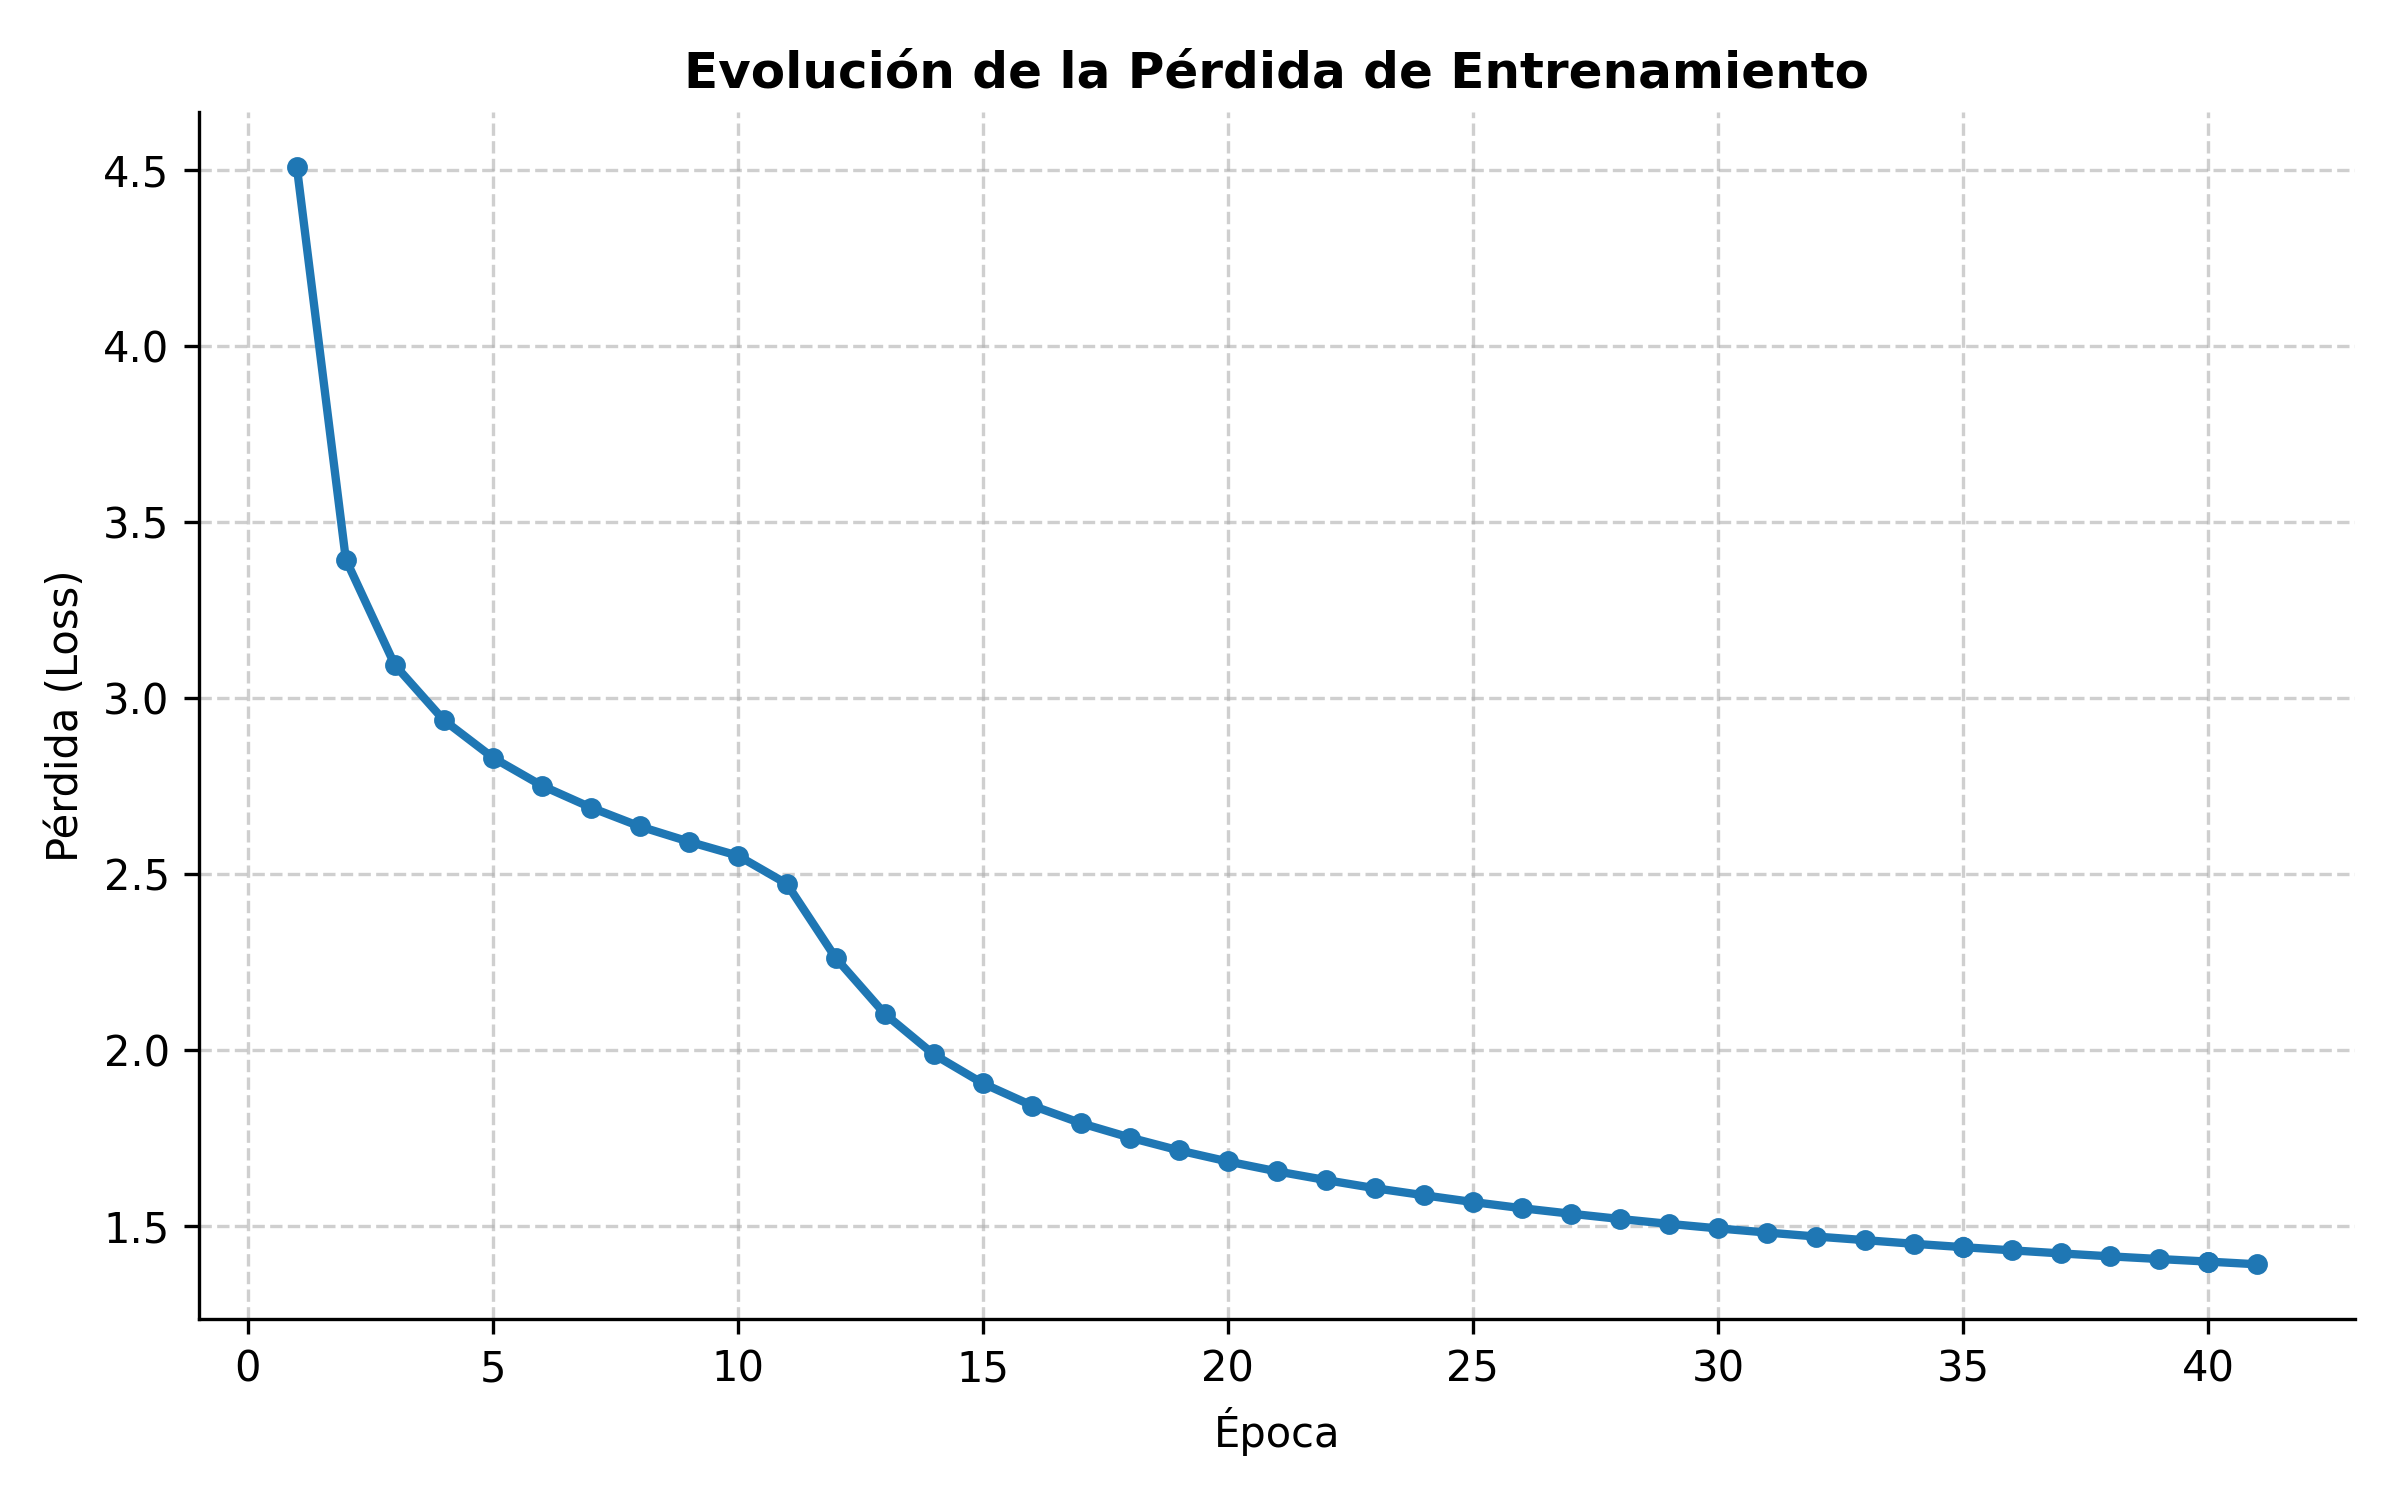
\includegraphics[width=0.7\textwidth]{Imagenes/train_loss.png}
    } 
    \hfill
    % --- LOSS VAL ---
    \subfloat[Evolución de la pérdida de validación.\label{subfig:hist_es}]{
        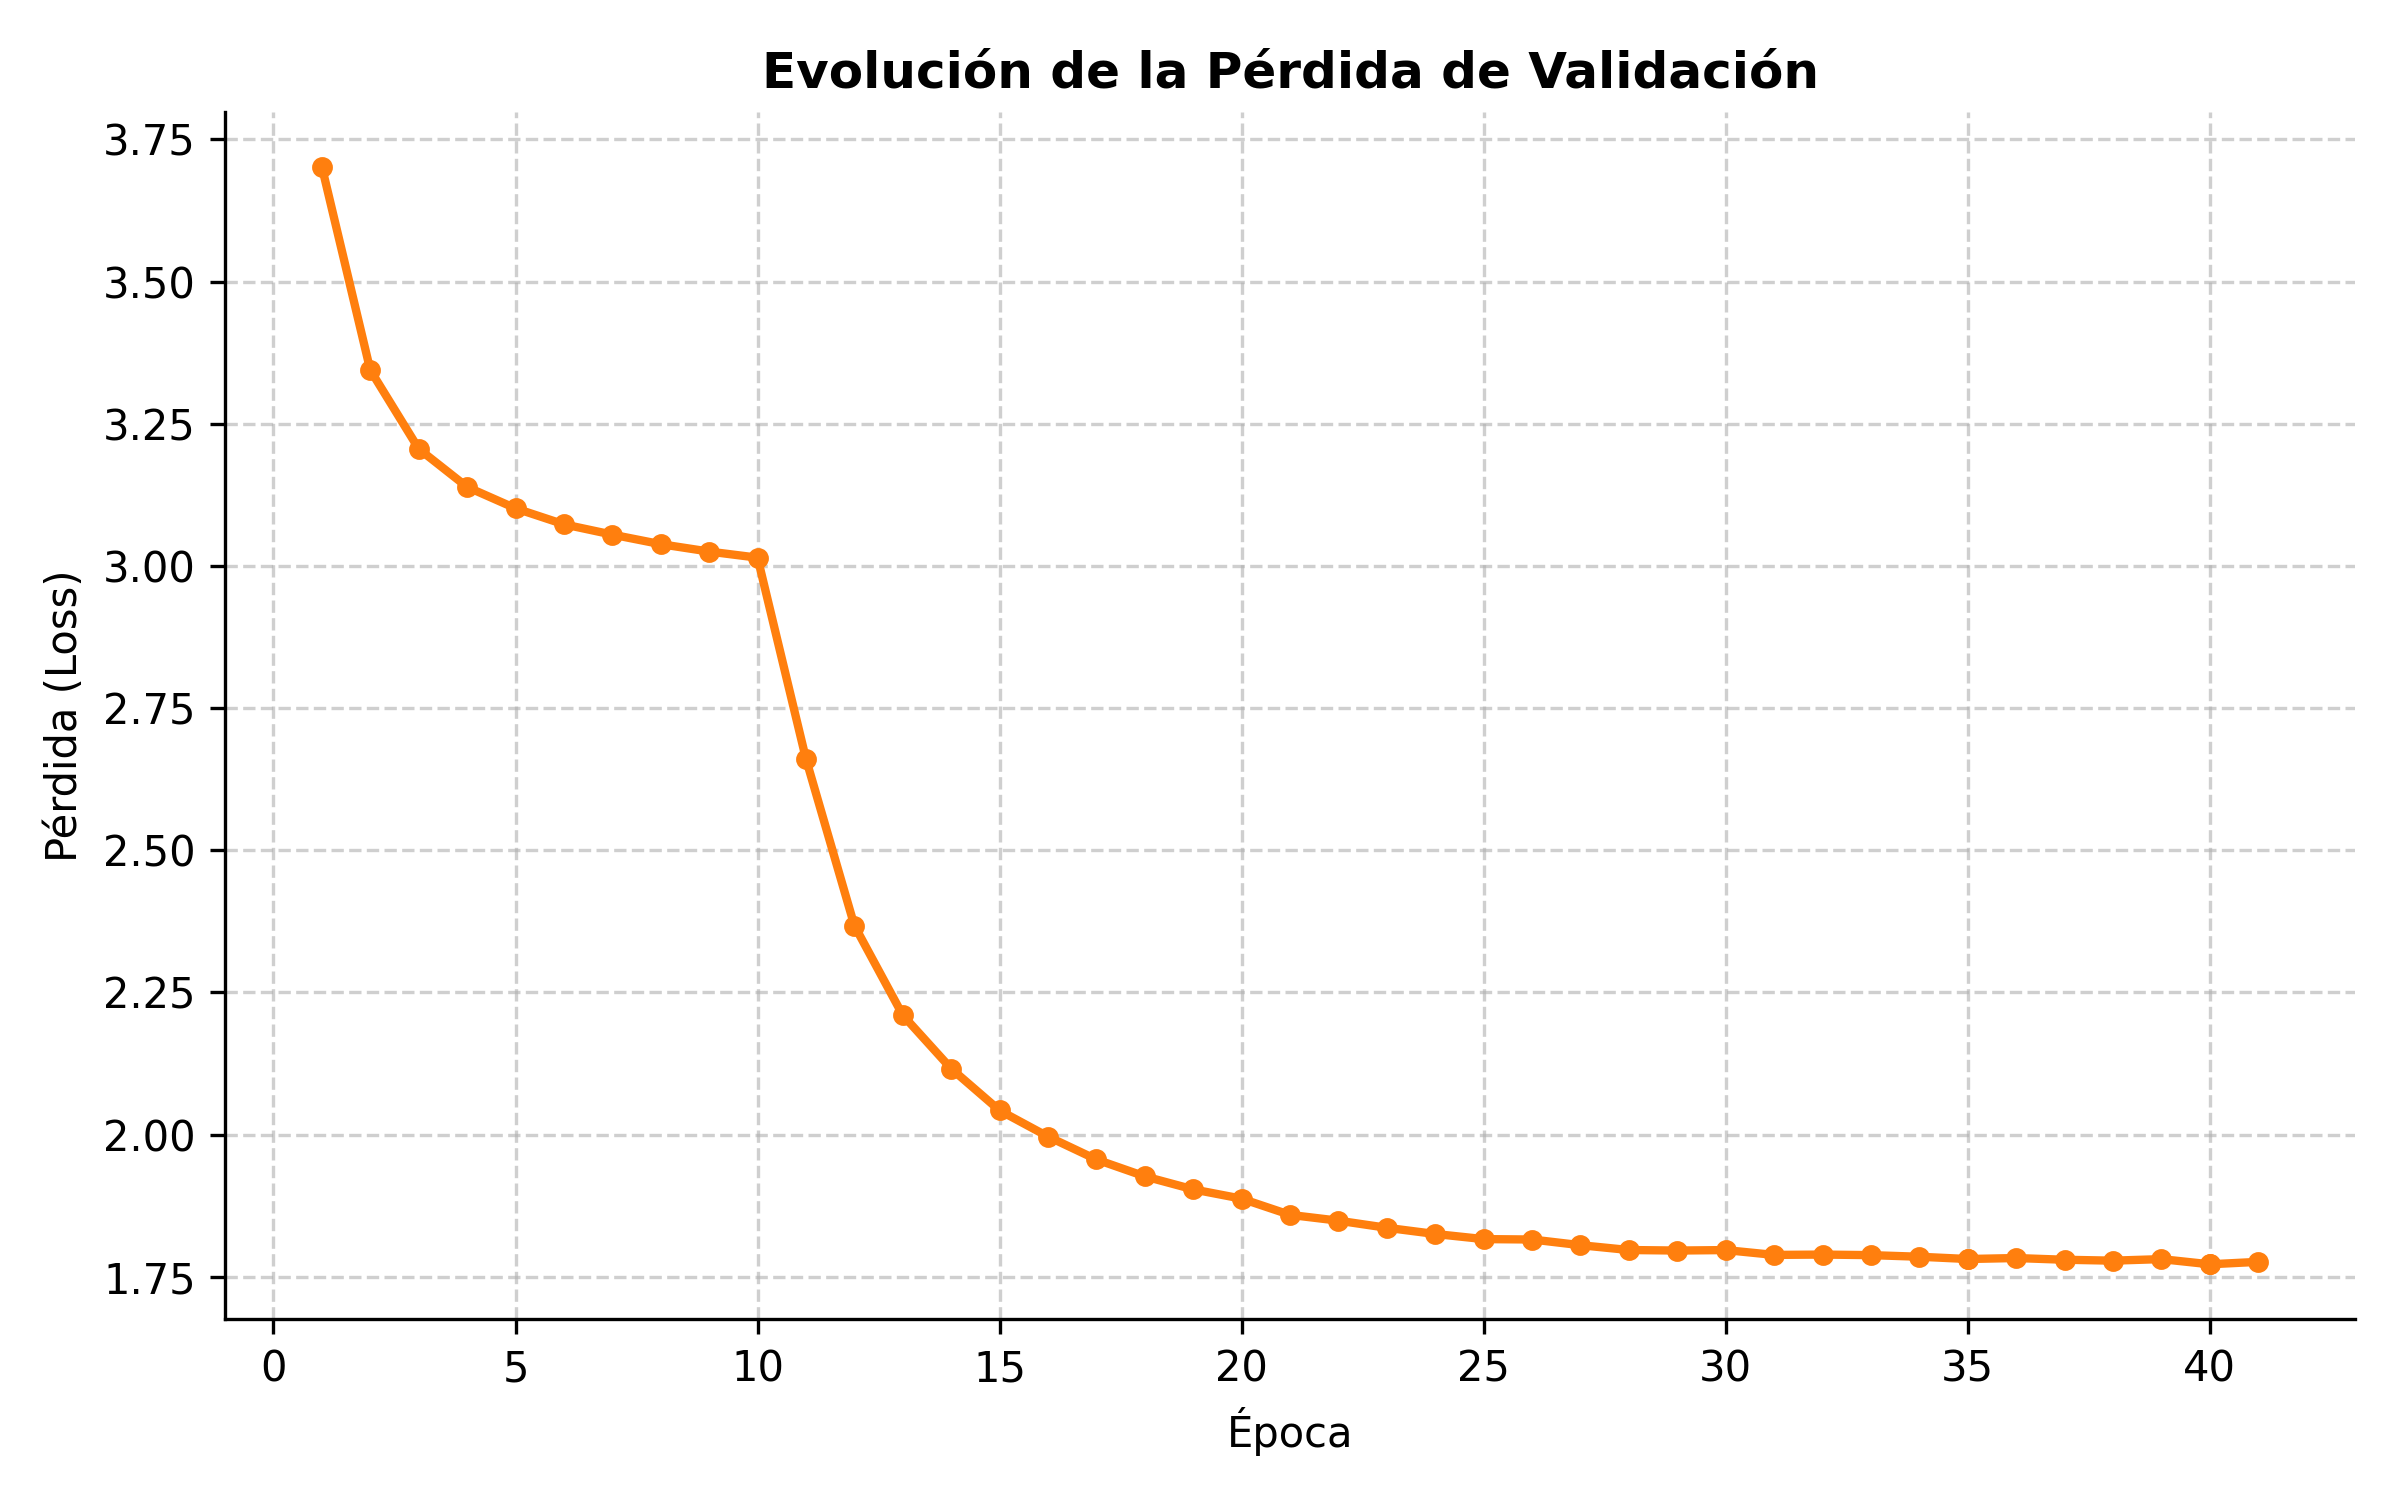
\includegraphics[width=0.7\textwidth]{Imagenes/val_loss.png}
    }

    \vspace{1em} % Espacio vertical entre filas

    \caption{Evolución de la función de pérdida $L$ calculada como el promedio sobre los respectivos conjuntos. El descenso simultáneo 
    en ambas curvas, considerando que los conjuntos de entrenamiento y validación son disjuntos, es un indicador de que el modelo está 
    aprendiendo y no simplemente memorizando los datos. En las etapas finales de la curva b) se intuye que el modelo converge y que continuar 
    el entrenamiento no mejorará significativamente el rendimiento. Es por ello que se decidió parar el entrenamiento, aunque inicialmente el 
    planteamiento era entrenar durante $50$ épocas.}
\label{fig:loss}
\end{figure}

\subsubsection{Optimización Mediante AdamW}

La actualización de los parámetros de la red se realiza mediante el algoritmo \textit{AdamW}, una extensión del descenso de gradiente 
estocástico que incorpora momentos de primer y segundo orden para adaptar la tasa de aprendizaje de forma individual para cada peso. 
Matemáticamente, este optimizador mejora la generalización del modelo al desacoplar el decaimiento de los pesos (\textit{weight decay}) de 
la actualización del gradiente. Se han mantenido los valores de diseño originales: $\beta_1 = 0.9$, $\beta_2 = 0.98$ y un factor de 
estabilidad $\epsilon = 10^{-9}$ para evitar divisiones por cero en el cálculo de las medias móviles.

\subsection{Planificación de la tasa de aprendizaje}

El entrenamiento de la arquitectura del transformador es altamente sensible a la selección de la tasa de aprendizaje ($\eta$). 
Por este motivo, en lugar de emplear un valor constante durante todo el proceso, se utiliza un planificador dinámico que ajusta este 
hiperparámetro en función del paso actual\footnote{Un paso se define cómo cada iteración de actualización de los parámetros del modelo 
tras procesar un lote (\textit{batch}) de datos.}. Matemáticamente, el comportamiento de $\eta$ se rige por la siguiente expresión:
\begin{equation}
    \eta = \frac{1}{\sqrt{D_{i}}} \cdot \min \left( \frac{1}{\sqrt{paso_{actual}}}, paso_{actual} \cdot calentamiento^{-1,5} \right)
\end{equation}
donde $D_{i}$, recordemos, representa la dimensión de los vectores $\x_n$ y $calentamiento$ es un valor predefinido que marca la duración de la 
fase inicial que, en nuestro caso, es 4.000. Esta función permite que el entrenamiento transcurra a través de dos etapas 
claramente diferenciadas:

\begin{itemize}
    \item \textbf{Fase de calentamiento:} Durante los primeros 4000 pasos, el segundo término de la ecuación domina el cálculo, lo que provoca 
    que la tasa de aprendizaje aumente de forma lineal desde cero. Este incremento progresivo es fundamental para la estabilidad del modelo en 
    sus fases iniciales, ya que evita que los gradientes inestables, propios de unos pesos todavía aleatorios, provoquen que el entrenamiento 
    diverja prematuramente.
    \item \textbf{Fase de decaimiento:} Una vez que el $paso\_actual$ supera el umbral de $calentamiento$, el primer término de la función se 
    vuelve dominante. A partir de este punto, la tasa de aprendizaje comienza a reducirse de forma proporcional a la raíz cuadrada inversa 
    del paso. Este descenso paulatino permite que el modelo realice ajustes cada vez más sutiles y precisos, facilitando una convergencia 
    óptima hacia el mínimo de la función de pérdida.
\end{itemize}



%==========================================
%METODOLOGIA
%==========================================
\subsection{Metodología de trabajo y experiencia personal}

La implementación del modelo se ha realizado íntegramente en PyTorch. Aunque ya contaba con experiencia previa en el 
desarrollo de redes neuronales, especialmente con arquitecturas convolucionales, este proyecto supuso un reto técnico 
distinto. La mayor dificultad no reside tanto en programar la lógica teórica, sino en gestionar correctamente el flujo y 
las dimensiones de los tensores a lo largo de toda la red. En PyTorch, el rendimiento depende de aprovechar el 
paralelismo de las funciones matriciales y evitar bucles secuenciales, lo que obliga a tener un control absoluto sobre 
cómo cambia la forma de los datos en cada capa.


Antes de comenzar a escribir el código, realicé una labor de investigación para estudiar otras implementaciones 
existentes. Dado que internet ofrece una cantidad ingente de ejemplos, fue necesario hacer un filtrado de calidad para 
seleccionar referencias fiables. Como base principal, utilicé el trabajo de Andrej Karpathy 
\cite{karpathy2023gpt_scratch}, una de las figuras más influyentes en el campo de la inteligencia artificial, exdirector 
de IA en Tesla y cofundador de OpenAI. Su enfoque educativo para construir transformadores desde cero permitió asentar 
las bases de este traductor. También fue fundamental el libro interactivo \textit{Dive into Deep Learning} 
\cite{zhang2023dive}, un recurso desarrollado por científicos de Amazon y diversas universidades que destaca por conectar 
de forma brillante la teoría matemática con su aplicación práctica en Python.


En cuanto al uso de herramientas de apoyo, utilicé modelos de lenguaje como Gemini y Claude. Sin embargo, no se emplearon 
para generar el código de forma automática, sino como una fuente de documentación dinámica: en caso de duda sobre el 
comportamiento de alguna función específica de PyTorch o sus argumentos, estos modelos permitían una consulta rápida y 
contrastada. Además, Claude resultó de gran utilidad para construir pequeños tests de prueba para cada componente de la 
red, asegurando que cada módulo funcionase correctamente antes de integrarlo en la estructura global.


Finalmente, debido al enorme coste computacional que implica entrenar un transformador, fue necesario recurrir a 
hardware especializado. Por su facilidad de uso, opté por la versión de pago de Google Colab, una plataforma basada en 
la nube que permite el acceso a tarjetas gráficas (GPU) de alto rendimiento. Para este trabajo, se adquirió un paquete 
de 100 unidades de computación que equivalen, aproximadamente, a unas 20 horas de uso. Aproximadamente la mitad se 
utilizó en las fases iniciales de pruebas y corrección de errores, mientras que las últimas 50 unidades se utilizaron 
para el entrenamiento final una vez ajustados todos los hiperparámetros, el dataset y el vocabulario. Esta gestión 
eficiente de los recursos fue clave, ya que en modelos de este tipo, optimizar la manipulación de los tensores es 
vital para no desperdiciar tiempo de computación y lograr que el sistema aprenda dentro de los límites disponibles.




%==========================================
%RESULTADOs
%==========================================
\subsection{Resultados}

Aunque existen métricas estandarizadas para evaluar el rendimiento de los modelos de traducción automática, en este proyecto se ha optado por 
realizar una evaluación cualitativa de diseño propio adaptada a nuestro enfoque unidireccional. El objetivo de esta prueba no es arrojar métricas 
con significancia estadística o rigor científico a gran escala, sino proporcionar una muestra representativa y empírica de cómo se comporta 
el modelo en la práctica. 

Para ello, se ha confeccionado un conjunto de pruebas compuesto por un total de 60 frases, distribuidas equitativamente (10 frases por categoría) 
entre los seis niveles de competencia lingüística del Marco Común Europeo de Referencia para las lenguas (A1, A2, B1, B2, C1 y C2). 
Esta estrategia permite observar, de manera exploratoria e intuitiva, la capacidad de la red para gestionar diferentes grados de complejidad 
gramatical y riqueza de vocabulario.

% ==========================================
% TABLA NIVEL A1
% ==========================================
\begin{table}[t!]
    \centering
    \begin{tabular}{p{0.47\textwidth} p{0.47\textwidth}}
        \toprule
        \textbf{Inglés (Original)} & \textbf{Español (Traducción)} \\
        \midrule
        I live in a small house. & Vivo en un pequeño hogar. \\
        My name is John and I am a student. & Mi nombre será John y yo, y soy estudiante. \\
        Do you like red apples? & - ¿Te gustan las manzanas rojas? \\
        She works in a big hospital. & Trabaja en un gran hospital. \\
        The book is on the table. & El libro se encuentra en la mesa. \\
        We play football every weekend. & Juguemos el fútbol todos los fines de semana. \\
        He is very happy today. & Hoy está muy contenta. \\
        They have a fast car. & Tienen un auto rápido. \\
        What time is it now? & ¿Qué hora es ahora? \\
        I want to drink cold water. & Quiero beber agua fría. \\
        \bottomrule
    \end{tabular}
    \caption{Evaluación cualitativa de traducción - Nivel A1.}
    \label{tab:evaluacion_A1}
\end{table}

% ==========================================
% TABLA NIVEL A2
% ==========================================
\begin{table}[t]
    \centering
    \begin{tabular}{p{0.47\textwidth} p{0.47\textwidth}}
        \toprule
        \textbf{Inglés (Original)} & \textbf{Español (Traducción)} \\
        \midrule
        I went to the cinema with my friends yesterday. & Fui al cine con mis amigos ayer. \\
        She is going to visit her grandmother next week. & Ella va a visitar a su abuela la próxima semana. \\
        We didn't buy any bread at the supermarket. & No compramos pan por el supermercado. \\
        Can you help me with my homework, please? & ¿Puedes ayudarme con mis tareas? \\
        He is taller than his older brother. & Es más alto que su hermano mayor. \\
        I enjoy listening to music when I walk to school. & Yo disfruto escuchar música cuando yo voy a las clases. \\
        The weather was very cold and it rained all day. & El tiempo era frío, la orejó todo el día. \\
        You must wear a uniform to work. & Debe llevar un uniforme al trabajo. \\
        Have you ever been to Paris? & ¿Has estado alguna vez en París? \\
        They are watching a funny movie on television. & Están mirando una película graciosa en televisión. \\
        \bottomrule
    \end{tabular}
    \caption{Evaluación cualitativa de traducción - Nivel A2.}
    \label{tab:evaluacion_A2}
\end{table}

% ==========================================
% TABLA NIVEL B1
% ==========================================
\begin{table}[t]
    \centering
    \begin{tabular}{p{0.47\textwidth} p{0.47\textwidth}}
        \toprule
        \textbf{Inglés (Original)} & \textbf{Español (Traducción)} \\
        \midrule
        If it rains tomorrow, we will probably stay at home and watch a movie. & Si sucede mañana, probablemente quedaremos en casa y veremos una película. \\
        I have been learning English for three years, but I still make mistakes. & He estado aprendiendo inglés durante tres años, pero todavía me equivoco. \\
        She told me that she had already finished the report before the meeting. & Me dijo que ya había terminado su reporte antes del encuentro. \\
        The museum, which was built in the 19th century, is currently closed. & El museo, construido en el siglo XIX, está actualmente cerrada. \\
        I used to play the piano when I was younger, but I don't have time anymore. & Antes jugaba por el piano cuando era más joven, pero ya no tengo tiempo. \\
        You shouldn't drink so much coffee because it might keep you awake. & No deberías beber mucho café porque podría mantenerte despierto. \\
        We are looking forward to spending our holidays at the beach this summer. & Estamos deseando estar en nuestra fiesta en la playa en este verano. \\
        The thieves were caught by the police while they were trying to escape. & Los ladrones fueron capturados por la policía mientras estaban tratando de escapar. \\
        Despite the heavy traffic, we managed to arrive at the airport on time. & A pesar del tráfico pesado, conseguimos llegar al aeropuerto a tiempo. \\
        Do you mind if I open the window to let some fresh air in? & ¿Te importa si abro las ventanas para dejar un poco de aire fresco? \\
        \bottomrule
    \end{tabular}
    \caption{Evaluación cualitativa de traducción - Nivel B1.}
    \label{tab:evaluacion_B1}
\end{table}

% ==========================================
% TABLA NIVEL B2
% ==========================================
\begin{table}[t]
    \centering
    \begin{tabular}{p{0.47\textwidth} p{0.47\textwidth}}
        \toprule
        \textbf{Inglés (Original)} & \textbf{Español (Traducción)} \\
        \midrule
        The new policy is expected to bring about significant changes in the economy. & Se espera que la nueva política lleve a cabo los cambios significativos en la economía. \\
        Had I known about the severe weather, I would have postponed my trip. & Me hubiera pasado por lo grave que tenía que haber puesto en mi viaje. \\
        She is highly regarded by her colleagues for her outstanding leadership skills. & Es muy considerado por sus colegas por sus habilidades de liderazgo. \\
        It goes without saying that hard work and dedication are crucial for success. & Va sin decir que la trabajadora de los más difícil es un logro crucial para el éxito. \\
        The company's profits have soared recently, largely due to a marketing campaign. & Los beneficios de la empresa han sufrido recientemente, principalmente debido a su campaña de comercialización. \\
        Not only did they fail to meet the deadline, but they also refused to apologize. & No solamente rechazaron el plazo, sino que también se negaron a disculparse. \\
        By the time we graduate next year, we will have completed all the coursework. & Para el momento de graduarse el año próximo, tendremos todo el transcurso. \\
        Taking all factors into consideration, the board has decided to approve the merger. & El Consejo ha decidido aprobar los factores de la fusión. \\
        I'm afraid I don't quite see eye to eye with you on this particular issue. & Me temo que no veo muy ojos en este asunto particular. \\
        The government has pledged to crack down on illegal dumping of hazardous waste. & El Gobierno ha prometido caer sobre el vertido ilícito de residuos peligrosos. \\
        \bottomrule
    \end{tabular}
    \caption{Evaluación cualitativa de traducción - Nivel B2.}
    \label{tab:evaluacion_B2}
\end{table}

% ==========================================
% TABLA NIVEL C1
% ==========================================
\begin{table}[t]
    \centering
    \begin{tabular}{p{0.47\textwidth} p{0.47\textwidth}}
        \toprule
        \textbf{Inglés (Original)} & \textbf{Español (Traducción)} \\
        \midrule
        Scarcely had the minister begun his speech when the protesters started chanting. & El Ministro apenas había iniciado su discurso cuando los manifestantes empezaron a cantar. \\
        The intricate plot of the novel is underscored by a profound existential dread. & El plegado intrínseco de la novela es recortizado por una profunda hilo de reflexión. \\
        The sweeping reforms implemented by the administration have drawn fierce criticism. & Las reformas dulces aplicadas por la administración han atraído críticas de gran resistencia. \\
        It is of paramount importance that we address the underlying causes of inequality. & Es sumamente importante que nosotros abordemos las causas subyacentes de la inequidad. \\
        To put it bluntly, their handling of the crisis was nothing short of disastrous. & Para darle una gran sensación de que la crisis no ha tenido ningún riesgo. \\
        The candidate's ambiguous stance on environmental issues ultimately cost him the election. & El candidato es un ambiguo punto ambiente de que a finales de los aspectos medioambientales le costó la elección. \\
        The findings of the longitudinal study corroborate the hypothesis posited earlier. & Ensayó sobre la evaluación de los análisis de longitudinal de la corroboró la hipótesis planteada anteriormente. \\
        Given the current economic climate, investing in volatile markets is tantamount to gambling. & Habida cuenta del actual clima económico en los mercados, invertir en los mercados de libre tamaño es una contribución a la juego. \\
        The artist's avant-garde exhibition challenges our preconceived notions of aesthetics. & La búsqueda de avant-garde presenta nuestras preconcebidas nociones de anesics. \\
        What I find most baffling is their sheer reluctance to embrace technological advancements. & Yo encuentro que la mayoría de los inconvenientes es su ferviente renuencia para abrazar avances tecnológicos. \\
        \bottomrule
    \end{tabular}
    \caption{Evaluación cualitativa de traducción - Nivel C1.}
    \label{tab:evaluacion_C1}
\end{table}

% ==========================================
% TABLA NIVEL C2
% ==========================================
\begin{table}[t]
    \centering
    \begin{tabular}{p{0.47\textwidth} p{0.47\textwidth}}
        \toprule
        \textbf{Inglés (Original)} & \textbf{Español (Traducción)} \\
        \midrule
        The sheer audacity of the embezzlement scheme left financial regulators utterly astounded. & La audición de la borda del esquema de encarnamiento dejó de los reguladores económicos importados de forma más agravante. \\
        Her seminal thesis systematically dismantles the fallacies prevalent in pedagogical discourse. & Sus tesis seminales dismo sistemáticamente las consecuencias previas prevalecen en los discursos pedagógicos. \\
        Amidst the cacophony of partisan bickering, his erudite arguments provided a beacon of rationality. & Amidst the Cacophony of partisan, sus argumentos eruditos dieron lugar al bacona de racionalidad. \\
        The treaty is fraught with legal ambiguities that could potentially precipitate international arbitration. & El tratado está a su vez consecuentes con ambigüedades jurídicas que podrían precipitar la arbitraje internacional. \\
        The author masterfully weaves a tapestry of disparate narratives into a cohesive magnum opus. & El autor es más autorizado de aislamiento a un escudo de narrativas en un opio cohesivo. \\
        It is a fundamental misconception to conflate correlation with causation in epidemiological studies. & Es una equivocación fundamental a la confusión de la correlación con causa de las causas en estudios epidemiológicos. \\
        The draconian austerity measures precipitated a rapid deterioration of the socioeconomic fabric. & El dliticio de austeridad determinó la rápida deterioro del tejido socioeconómico. \\
        His esoteric references, though intellectually stimulating, often alienated the layperson. & Sus referencias esotéricas, aunque intelectualmente estimulantes, muchas veces alienadas. \\
        The insidious nature of the malware allowed it to circumvent cryptographic defenses with impunity. & La insidiosa naturaleza del Malware se le permite circuncidar las defensas racionales de muerte de forma asfixiante. \\
        Bereft of all hope, the protagonist is thrust into a maelstrom of moral ambiguity. & A menudo de todos los esperaban que el protagonista se apresurara al de la ambigüedad moral. \\
        \bottomrule
    \end{tabular}
    \caption{Evaluación cualitativa de traducción - Nivel C2.}
    \label{tab:evaluacion_C2}
\end{table}


Los resultados de esta prueba (ver tablas \ref{tab:evaluacion_A1}, \ref{tab:evaluacion_A2}, \ref{tab:evaluacion_B1}, \ref{tab:evaluacion_B2}, 
\ref{tab:evaluacion_C1} y \ref{tab:evaluacion_C2}) muestran de forma muy clara cómo se comporta el modelo: es capaz de defenderse con el 
inglés cotidiano, pero sufre notablemente cuando el texto se vuelve complejo. 

En los niveles básicos (A1 y A2), se observa que la red ha aprendido bien la estructura general de las frases. Es capaz de traducir oraciones 
directas sin problema, como al pasar de ``I live in a small house'' a ``Vivo en un pequeño hogar''. Sin embargo, ya se aprecian descuidos con 
el género y el número; por ejemplo, traduce el masculino ``He is very happy'' como ``Hoy está muy contenta'' o se refiere al museo como 
``cerrada''. También aparece la primera palabra inventada al traducir que llovió todo el día usando el verbo ``orejó''.

A medida que pasamos a los niveles intermedios (B1 y B2), la dificultad aumenta por el uso de tiempos verbales más complejos y frases hechas. 
Aquí el modelo peca de traducir literalmente palabra por palabra. Esto hace que fracase al traducir palabra por palabra frases hechas como 
``see eye to eye'' traducida a ``no veo muy ojos'', cuando su significado real es ``estar de acuerdo''. También demuestra falta de contexto 
al traducir ``play the piano'' como ``jugaba por el piano'' en lugar de tocar, y se pierde por completo cuando la estructura gramatical se 
invierte, como ocurre con ``Had I known about...'', perdiendo el sentido de la frase original.

Finalmente, en los niveles avanzados (C1 y C2), el modelo sencillamente colapsa. Al encontrarse con vocabulario muy específico o poco común 
que apenas habrá visto en su fase de entrenamiento, empieza a alucinar texto. Por un lado, se inventa palabras que suenan parecido al español 
pero que no existen, como ``recortizado'', ``dismo'' o ``bacona''. Por otro lado, intenta adivinar términos complejos basándose en sus primeras 
letras, lo que provoca el fallo más llamativo de toda la prueba: traducir ``circumvent'' (esquivar o eludir) por ``circuncidar'', lo que arrastra 
al resto de la oración a no tener ningún sentido.

En resumen, la prueba demuestra que el traductor funciona correctamente para un uso básico y literal. Sin embargo, para alcanzar una competencia 
lingüística de nivel nativo, sería necesario ampliar significativamente el conjunto de datos de entrenamiento, permitiendo a la red exponerse a 
una mayor variedad de estructuras complejas y vocabulario técnico. También modificar la arquitectura hacia un modelo de traducción bidireccional 
podría mejorar los resultados. Pues a diferencia del modelo actual, que procesa la información de unidireccional, un modelo bidireccional analiza 
la oración completa en ambos sentidos antes de traducirla, es decir, el codificador recibe y codifica ambas frases antes de traducirla. 
Esto permite que el mecanismo de atención capture el contexto global, entendiendo cómo el final de una frase puede cambiar el sentido del 
principio. Esta visión de conjunto es lo que permitiría al modelo identificar frases hechas o dobles sentidos, evitando traducciones literales 
erróneas y resolviendo ambigüedades que solo se aclaran al leer la oración en su totalidad.


\section{Detalles de implementación}

Existen ciertos aspectos técnicos que, aunque fundamentales para el funcionamiento del modelo, se han reservado para este capítulo con el 
objetivo de agilizar la exposición teórica de las secciones anteriores.

\subsection{Escalado del producto escalar}

El primer detalle de implementación se centra en la ecuación de atención descrita en el capítulo 3 (ver \ref{eq:eq_transformer}). En el artículo 
original, la función de atención se redefine mediante la introducción de un factor de escalado $1/\sqrt{D_i}$:
\begin{equation}
    \text{Attention}(\mathbf{Q}, \mathbf{K}, \mathbf{V}) = \text{Softmax} \left( \frac{\mathbf{Q} \mathbf{K}^T}{\sqrt{D_i}} \right) \mathbf{V}
    \label{eq:eq_transformer_scaled}
\end{equation}
Donde $D_i$ representa la dimensionalidad de los vectores de entrada $\mathbf{x}_n$. Esta modificación responde a una necesidad práctica 
detectada por los autores, pues observaron que para valores elevados de $D_i$, el producto escalar tiende a crecer excesivamente en magnitud. 
Esto desplaza la función \textit{Softmax} hacia regiones de saturación donde el gradiente es extremadamente pequeño, lo que dificulta el 
entrenamiento del modelo y al dividir por $\sqrt{D_i}$, se contrarresta este efecto de magnitud, manteniendo los valores en un rango que permite 
que los gradientes fluyan correctamente sin que el mecanismo de atención se vea afectado o pierda capacidad de aprendizaje.

\subsection{Paralelismo y relleno (\textit{padding})}

El segundo detalle relevante tiene que ver con el aprovechamiento de la potencia de cómputo. El uso de tarjetas gráficas (GPU) en el ámbito de 
la inteligencia artificial se justifica por su capacidad para procesar grandes volúmenes de datos en paralelo. Para explotar esta arquitectura, 
es estrictamente necesario que los datos se organicen en bloques o lotes (\textit{batches}) de dimensiones homogéneas. 

En nuestro caso, el procesamiento de lenguaje natural, nos enfrentamos al problema de que las frases tienen longitudes variables. En consecuencia, 
para que todas las frases de un lote tengan la misma dimensión y puedan ser procesadas simultáneamente por la GPU, se introduce el concepto de 
relleno (\textit{padding}) el cual utiliza un \textit{token} especial denominado \texttt{<PAD>}, perteneciente al vocabulario $\mathcal{V}$, 
para completar las frases más cortas hasta alcanzar una longitud máxima predefinida (en este proyecto, $N = 128$).

Por ejemplo, si nuestra longitud máxima es 6 y tenemos la frase ``Me gusta el café'', la representación con relleno, considerando palabras 
como \tokens{}, sería:
\begin{center}
    \texttt{[Me, gusta, el, café, <PAD>, <PAD>]}
\end{center}


Sin embargo, la introducción de \textit{tokens} de relleno genera un inconveniente: el modelo podría aprender que el \textit{token} \texttt{<PAD>} 
es una parte fundamental de la semántica de la frase debido a su alta frecuencia de aparición y podría dar a  luegar a que el modelo aprendiese, 
única y exclusivamente, a predecir frases compuestas solo por el \token{} \texttt{<PAD>}. Para evitar que el mecanismo de atención preste atención 
a este nuevo \token{}, se aplica una máscara de relleno antes de la función \textit{Softmax}.

Esta máscara de relleno no es más que  añadir una matriz de máscara $\textbf{M}$ al producto de las consultas y claves ($\mathbf{Q}\mathbf{K}^T$) 
y cuyos valores son  $-\infty$ en todas las posiciones que corresponden a un \textit{token} de relleno y $0$ en caso contrario:
\begin{equation}
    \text{Attention}(\mathbf{Q}, \mathbf{K}, \mathbf{V}) = \text{Softmax} \left( \frac{\mathbf{Q} \mathbf{K}^T + \textbf{M}}{\sqrt{D_i}} \right) 
    \mathbf{V}
\end{equation}
Dado que cualquier valor al que se le suma $-\infty$ da como resultado $-\infty$, al aplicar la función \textit{Softmax} ($e^{-\infty} = 0$), 
las posiciones del relleno se anulan por completo. En consecuencia, el peso de atención sobre el relleno es cero, garantizando que estos 
\textit{tokens} no afecten al cálculo de los pesos del resto de la secuencia.

En conclusión, al introducir esta máscara de relleno en la ecuación de atención, conseguimos que el modelo ignore los datos vacíos y se centre 
solo en la información útil de cada frase. Al estandarizar la longitud de las secuencias de esta manera, podemos procesar los datos en lotes 
aprovechando toda la potencia de cálculo de las tarjetas gráficas. Esto no solo mejora la calidad del aprendizaje, sino que acelera 
considerablemente el entrenamiento al explotar el paralelismo del hardware, permitiendo obtener resultados en  menos tiempo.



